\section{Versuchsauswertung}

\subsection{Versuch 1}
Im ersten Versuchsteil wurden sechs verschiedene Durchflüsse von \SI{60}{\liter\per\hour} bis \SI{660}{\liter\per\hour} mit Hilfe eines Taco-Setters eingestellt und die Messdaten der verbauten Sensoren verglichen. Als Referenz wurde das durchströmende Wasser am Auslass der Messstrecke in einem Eimer gesammelt, gewogen und die Messdauer notiert. Dieser Wert wird als wahrer Durchfluss angenommen. Abbildung \ref{fig:devPc} zeigt die Abweichung der unterschiedlichen Sensoren vom wahren Durchfluss. 

\begin{figure}[H]
	\centering
	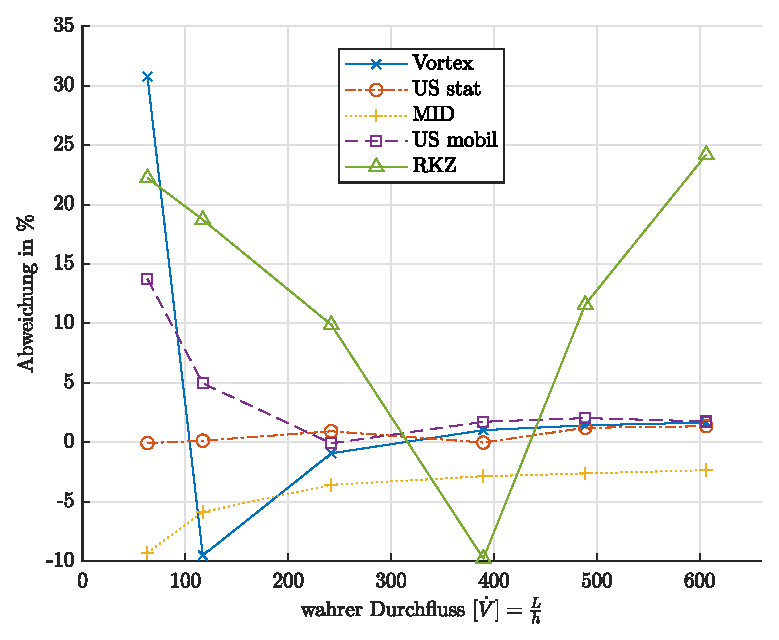
\includegraphics[width=0.8\textwidth]{../DATA/devPcPlot.eps}
	\caption[Messabweichung Sensoren]{Auftragung der Messabweichung verschiedener Sensoren bei definierten Volumenströmen vom wahren Wert.}
	\label{fig:devPc}
\end{figure}

\begin{table}[H]
	\centering
	\caption[Arithmetische Mittelwerte und Standardabweichungen der Durchflusssensoren.]{Arithmetische Mittelwerte und Standardabweichungen der Durchflusssensoren. (MID = Magnetisch induktiver Durchflussmesser, US = Ultraschall, RKZ = Ringkolbenzähler)}
	\label{tab:meanSigData}
	\begin{tabular}{S[separate-uncertainty,table-parse-only,table-figures-uncertainty = 1]S[separate-uncertainty,table-parse-only,table-figures-uncertainty = 1]S[separate-uncertainty,table-parse-only,table-figures-uncertainty = 1]S[separate-uncertainty,table-parse-only,table-figures-uncertainty = 1]}
		
		
		
		{wahrer Durchfluss}        &  {Vortex}            &{US stat}            &{MID}            \\  
		{$[\dot{V}] = \si{\litre\per\hour}$}&{$[\dot{V}] = \si{\litre\per\hour}$}&{$[\dot{V}] = \si{\litre\per\hour}$}&{$[\dot{V}] = \si{\litre\per\hour}$}\\
		\midrule
		63(2)               &  43.7  (24  ) & 63.2  (  10) &  69.0  ( 06 )  \\
		116(2)              &  128.1 ( 09  ) & 116.8 (  10) &  123.8 ( 08 )  \\
		241(2)               &  244.1 ( 11  ) & 239.6 (  10) &  250.4 ( 09 )  \\
		389(2)               &  385.8 ( 25  ) & 389.8 (195)  &  400.9 ( 22 )  \\
		488(2)               &  481.9 ( 18  ) & 482.9 (  15) &  501.6 ( 13 )  \\
		606(2)               &  596.4 ( 28  ) & 598.2 (  27) &  620.6 ( 33 )  \\
		\bottomrule
		{wahrer Durchfluss}&		{US mobil}       &    {RKZ}           				 & {Stichprobengröße} \\
		{$[\dot{V}] = \si{\litre\per\hour}$}&{$[\dot{V}] = \si{\litre\per\hour}$}&{$[\dot{V}] = \si{\litre\per\hour}$}& {$[n]$ = Stück}\\
		\midrule
		 63(2)	&  54.4  ( 14 ) &   49.1  ( 181) & 514\\
		116(2)	& 111.1  ( 12 ) &   95.0  ( 350) & 236\\
		241(2)	& 242.0  ( 08 ) &  217.9  ( 677) & 122\\
		389(2)	& 383.0  ( 30 ) &  427.8  (1323) &  83\\
		488(2)	& 478.9  ( 19 ) &  432.1  (1361) &  64\\
		606(2)	& 595.8  ( 31 ) &  459.7  (1865) &  49\\
		\bottomrule
	\end{tabular}
\end{table}


Die geringste Abweichung bietet das Stationäre Ultraschallgerät mit unter 2\% Abweichung über den gesamten Messbereich hinweg. Auch das mobile Ultraschallgerät bietet ab \SI{240}{\liter\per\hour} eine ähnliche Genauigkeit. Das MID bietet erst ab einem Durchfluss von \SI{300}{\liter\per\hour} eine konstante Genauigkeit bei einer Abweichung von -3\%. Der Vortexmesser ist mit einem minimalen Arbeitsbereich von \SI{50}{\liter\per\hour} angegeben, praktisch liefert er bei \SI{60}{\liter\per\hour} keinen brauchbaren Wert. Ab \SI{240}{\liter\per\hour} liefert er plausible Werte. Am schlechtesten schneidet der Ringkolbenzähler ab, welcher mit hohen Abweichungen im zweistelligen Bereich (je nach Durchflussrate in beide Richtungen) lediglich für qualitative Messungen geeignet ist. Die Problematik liegt hierbei in der Messmethode: Der Zähler gibt nur bei jedem ganzen Liter einen Impuls aus. Bei dem maximalen wahren Durchfluss von ca. \SI{600}{\liter\per\hour} entspricht dies einem Impuls alle sechs Sekunden. Bei geringeren Durchflüssen steigt der zeitliche Abstand zwischen den Impulsen. Je nach gewähltem Scanabschnitt bei der Auswertung variiert die Abweichung.
Für das Wägeverfahren wurde die Genauigkeit der Waage auf ganze Gramm geschätzt, die Unsicherheit bei der Zeitmessung auf eine Sekunde. Mit steigenden Durchflüssen (und kürzeren Messzeiten bis zur Füllung des Eimers) nimmt der Einfluss der Zeitmessung zu.

\subsection{Versuch 2}

%Tabelle mit den Messwerten anlegen

Abbildung \ref{fig:temp} zeigt den gemessenen Temperaturverlauf der beiden Sensoren.

\begin{figure}[H]
	\centering
	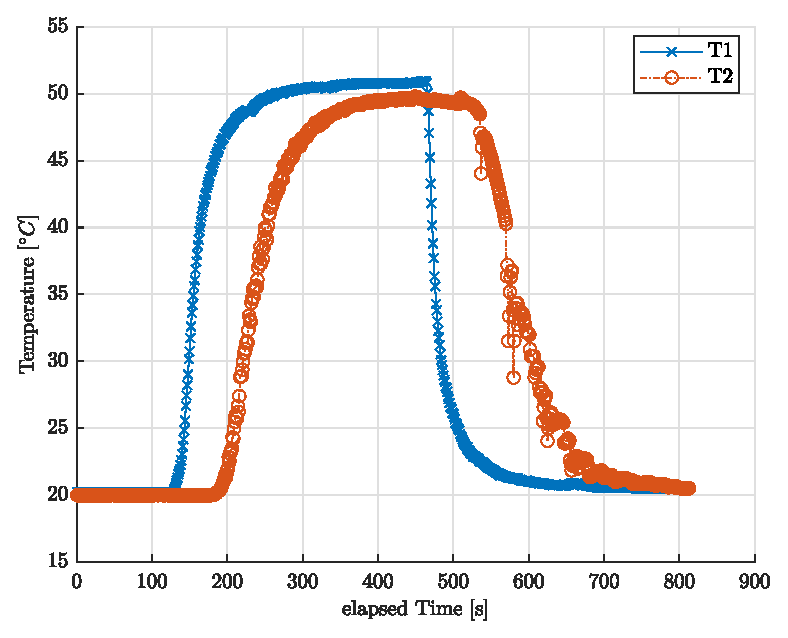
\includegraphics[width=0.8\textwidth]{../DATA/tempPlot.eps}
	\caption{Darstellung der gemessenen Temperatur über der Zeit}
	\label{fig:temp}
\end{figure}

Zur Bestimmung des Durchflusses wird  die Laufzeit (Zeitlicher Abstand der Flanken beider Verläufe) bestimmt. Dieser ist Abbildung \ref{fig:temp} zu entnehmen und abzuschätzen.

\begin{center}
	\begin{tabular}{l|c}
		\label{tab:}
		
		\textbf{Flanke} & \textbf{Laufzeit} [t] = s\\
		\hline
		steigend & 70$\pm$5 
	\end{tabular}
\end{center}

Für die Auswertung wird die steigende Flanke genutzt, da diese schärfer aufgelöst ist.

Die gemessene Strecke zwischen den beiden Sensoren beträgt 9,48$\pm$\si{\meter}, der Querschnitt der Leitung ist mit \SI{0,02}{\meter} angegeben. Das Volumen der Messstrecke berechnet sich nach Gleichung \ref{eq:vol} zu:

\begin{equation}
	\label{eq:vol}
	V_{\text{Rohr}} = \pi * r^2 * l = \pi * (\SI{0,01}{\meter})^2 * \SI{9,48}{\meter} = 2,978\pm0,0314\si{\litre}
\end{equation}

Der Durchfluss entspricht dem Quotienten aus Rohrvolumen und Laufzeit und ist in Gleichung \ref{eq:flow} berechnet.

\begin{equation}
	\label{eq:flow}
	\dot V = \frac{V_{Rohr}}{t_{LZ}}*\SI{3600}{\second\per\hour} = \frac{2,978\pm0,00314\si{\litre}}{70\pm5\si{\second}}*\SI{3600}{\second\per\hour} = 153\pm12\si{\litre\per\hour}
\end{equation}

Der MID hat während der Flankenmessung einen Durchfluss von \SI{234,4(48)}{\litre\per\hour} angezeigt, was \SI{53}{\percent} über dem experimentell bestimmten Wert liegt. Da es sich bei der Flankenmessung um ein thermisches Messverfahren handelt, ist dieses mit einer gewissen Latenz verbunden. Die Differenz zwischen den gemessenen Flanken sollte ohne diese Einschränkung kürzer ausfallen, wodurch ein höherer Volumenstrom resultiert. Die Längenmessung hat einen verhältnismäßig geringen Einfluss auf das Messergebnis und wurde mit einer Unsicherheit von \SI{10}{\centi\meter} geschätzt. Bei \SI{20}{\centi\meter} steigt die Unsicherheit des Ergebnisses auf \SI{14}{\litre\per\hour}. Da die Temperaturflanken eine gewisse Krümmung aufweisen, wurde hier eine Unsicherheit von 5 Sekunden angenommen. Die Zeit hat somit den größeren Einfluss auf die Messung. 


